% !TEX program = xelatex
\documentclass[aspectratio=169,11pt]{beamer}

\usepackage{fontspec}
\defaultfontfeatures{Ligatures=TeX,Scale=MatchLowercase}
\setsansfont{SourceSans3-Regular.otf}[
  BoldFont=SourceSans3-Semibold.otf,
  ItalicFont=SourceSans3-RegularIt.otf,
  BoldItalicFont=SourceSans3-SemiboldIt.otf]
\setmainfont{LibertinusSerif-Regular.otf}[
  BoldFont=LibertinusSerif-Semibold.otf,
  ItalicFont=LibertinusSerif-Italic.otf]
\setmonofont{IBMPlexMono-Regular.otf}[
  BoldFont=IBMPlexMono-SemiBold.otf,
  Scale=0.82]

\usepackage{graphicx}
\usepackage{booktabs,tabularx,array}
\usepackage{qrcode}
\usepackage{tikz}
\usetikzlibrary{arrows.meta,positioning,shapes.geometric,fit,calc}
\usepackage{amsmath}
\newcolumntype{Y}{>{\raggedright\arraybackslash}X}
\newcolumntype{M}[1]{>{\raggedright\arraybackslash}m{#1}}

\definecolor{hbgreen}{HTML}{087F78}
\definecolor{hbnavy}{HTML}{173C4A}
\definecolor{hbgold}{HTML}{B45309}
\definecolor{hbink}{HTML}{17211F}
\definecolor{hbmuted}{HTML}{50615C}
\definecolor{hbline}{HTML}{DDE5E1}
\definecolor{hblight}{HTML}{F4F8F6}

\setbeamercolor{normal text}{fg=hbink,bg=white}
\setbeamercolor{structure}{fg=hbgreen}
\setbeamercolor{frametitle}{fg=hbnavy,bg=white}
\setbeamercolor{title}{fg=white}
\setbeamercolor{subtitle}{fg=white}
\setbeamercolor{block title}{fg=hbnavy,bg=white}
\setbeamercolor{block body}{fg=hbink,bg=white}
\setbeamercolor{block title alerted}{fg=hbgold,bg=white}
\setbeamercolor{block body alerted}{fg=hbink,bg=white}
\setbeamercolor{alerted text}{fg=hbgold}
\usefonttheme{professionalfonts}
\setbeamerfont{normal text}{family=\sffamily}
\setbeamerfont{frametitle}{family=\sffamily,series=\bfseries,size=\Large}
\setbeamerfont{block title}{family=\sffamily,series=\bfseries}
\setbeamerfont{block body}{family=\sffamily}
\setbeamertemplate{navigation symbols}{}
\setbeamertemplate{itemize item}{\color{hbgreen}\small$\blacktriangleright$}
\setbeamertemplate{itemize subitem}{\color{hbnavy}\tiny$\bullet$}
\setbeamertemplate{frametitle}{%
  \vspace{0.2cm}
  \insertframetitle\par
  \vspace{0.05cm}
  {\color{hbgreen}\rule{\textwidth}{0.8pt}}
}
\setbeamertemplate{footline}{%
  \leavevmode
  \hbox{%
    \begin{beamercolorbox}[wd=.82\paperwidth,ht=2.7ex,dp=1.2ex,leftskip=.55cm]{author in head/foot}
      \color{hbmuted}\scriptsize HeapBeat \textbullet\ Đồ án Cấu trúc dữ liệu và Giải thuật
    \end{beamercolorbox}%
    \begin{beamercolorbox}[wd=.18\paperwidth,ht=2.7ex,dp=1.2ex,rightskip=.55cm plus1fil]{date in head/foot}
      \color{hbmuted}\scriptsize \insertframenumber/\inserttotalframenumber
    \end{beamercolorbox}%
  }
}

\newcommand{\code}[1]{\texttt{#1}}
\newcommand{\metricline}[1]{%
  {\sffamily\small\bfseries\color{hbgreen}#1}}

\title{HeapBeat}
\subtitle{Phát nhạc chờ cộng đồng cho phòng tự học (Collaborative DJ Queue)}
\author{Nhóm HeapBeat}
\date{Ngày 08 tháng 08 năm 2026}

\begin{document}

% 1 ---------------------------------------------------------------------------
\begin{frame}[plain,t]
\begin{tikzpicture}[remember picture,overlay]
  \fill[white] (current page.south west) rectangle (current page.north east);
  \fill[hbnavy] (current page.south west) rectangle
    ($(current page.north west)+(0.28cm,0)$);
  \fill[hblight] ($(current page.north west)+(0.28cm,0)$) rectangle
    ($(current page.north east)+(0,-1.45cm)$);
  \fill[hbgreen] ($(current page.south west)+(0.28cm,0)$) rectangle
    ($(current page.south east)+(0,0.1cm)$);
\end{tikzpicture}
\vspace*{0.06cm}
\begin{columns}[c,totalwidth=\textwidth]
\column{0.12\textwidth}

\includegraphics[width=1.2cm]{../report/logo-khtn.png}
\column{0.84\textwidth}
{\sffamily\scriptsize\color{hbnavy}ĐẠI HỌC QUỐC GIA TP.HCM\par}
{\sffamily\small\bfseries\color{hbnavy}TRƯỜNG ĐẠI HỌC KHOA HỌC TỰ NHIÊN\par}
{\sffamily\scriptsize\color{hbmuted}KHOA ĐIỆN TỬ -- VIỄN THÔNG\par}
\end{columns}
\vspace{0.34cm}
\color{hbnavy}
{\sffamily\scriptsize\bfseries\color{hbgreen}BÁO CÁO ĐỒ ÁN\par}
\vspace{0.06cm}
{\sffamily\small\bfseries CẤU TRÚC DỮ LIỆU VÀ GIẢI THUẬT\par}
\vspace{0.24cm}
{\fontsize{34}{37}\selectfont\bfseries HeapBeat\par}
\vspace{0.12cm}
{\Large\bfseries\color{hbgreen}Phát nhạc chờ cộng đồng cho phòng tự học\par}
\vspace{0.08cm}
{\small\bfseries\color{hbnavy}(COLLABORATIVE DJ QUEUE)\par}
\vspace{0.38cm}
{\scriptsize\bfseries\color{hbgreen}NHÓM SINH VIÊN THỰC HIỆN\par}
\vspace{0.12cm}
{\small
\renewcommand{\arraystretch}{1.14}
\begin{tabular}{@{}p{5.1cm}p{5.1cm}@{}}
Phạm Hùng Tiến & Phạm Cao Bằng\\
Trần Thái Nguyên & Lê Quang Bảo Trung\\
Quách Gia Thịnh & Văn Phú Duy\\
Đặng Gia Toàn & Hồ Sĩ Phú\\
\end{tabular}\par}
\vfill
\color{hbmuted}\scriptsize Thành phố Hồ Chí Minh, ngày 08 tháng 08 năm 2026
\end{frame}

% 2 ---------------------------------------------------------------------------
\begin{frame}{Bài toán là sắp xếp lựa chọn chung mà không để một người chi phối}
\begin{columns}[T,totalwidth=\textwidth]
\column{0.48\textwidth}
\begin{block}{Bối cảnh sử dụng}
\begin{itemize}
  \item Nhiều sinh viên tại sảnh hoặc phòng tự học muốn yêu cầu bài hát.
  \item Danh sách phát phải phản ánh lựa chọn chung.
  \item Việc chuyển bài và lặp danh sách phải liền mạch.
  \item Hệ thống phải ngăn gửi dồn, gửi trùng và phá hàng đợi.
\end{itemize}
\end{block}
\column{0.48\textwidth}
\begin{block}{Tiêu chí thiết kế}
\begin{itemize}
  \item Bài có điểm cao nhất luôn ở gốc Heap.
  \item Lịch sử phát là một vòng liên kết hai chiều.
  \item Mỗi StudentID có một trạng thái kiểm soát gửi yêu cầu.
  \item Chỉ bài có hồ sơ giấy phép mới được phát.
\end{itemize}
\end{block}
\end{columns}
\vspace{0.35cm}
\begin{center}
\metricline{Công bằng \quad\textbullet\quad phản hồi tức thời \quad\textbullet\quad có thể kiểm chứng
\quad\textbullet\quad tôn trọng quyền sử dụng}
\end{center}
\end{frame}

% 3 ---------------------------------------------------------------------------
\begin{frame}{Ba cấu trúc dữ liệu giải quyết ba thao tác cốt lõi}
\small
\renewcommand{\arraystretch}{1.48}
\setlength{\tabcolsep}{4pt}
\centering
\begin{tabular}{@{}M{2.35cm}M{2.45cm}M{5.25cm}M{2.55cm}@{}}
\toprule
\textbf{Thao tác} & \textbf{Cấu trúc} & \textbf{Kết quả trực tiếp} & \textbf{Chi phí}\\
\midrule
\shortstack[l]{Bình chọn\\bài kế tiếp} &
\shortstack[l]{\alert{Max-Heap}\\\alert{+ Map chỉ số}} &
Map định vị yêu cầu; Heap luôn giữ bài ưu tiên nhất tại gốc. &
\shortstack[l]{xem $O(1)$\\cập nhật $O(\log n)$}\\
\addlinespace[1mm]
\shortstack[l]{Next / Previous\\Repeat All} &
\alert{Circular DLL} &
Liên kết hai chiều và khép vòng; \code{addLast} nối bài vừa phát vào cuối. &
\shortstack[l]{di chuyển $O(1)$\\thêm cuối $O(1)$}\\
\addlinespace[1mm]
\shortstack[l]{Chặn spam\\thu hồi yêu cầu} &
\alert{Hash Map} &
StudentID ánh xạ trực tiếp tới cửa sổ gửi, trạng thái chặn và các requestId. &
\shortstack[l]{kiểm tra\\TB $O(1)$}\\
\bottomrule
\end{tabular}
\vspace{0.42cm}
\begin{center}
\metricline{Mỗi cấu trúc giữ một bất biến và một nhóm thao tác riêng}
\end{center}
\end{frame}

% 4 ---------------------------------------------------------------------------
\begin{frame}{Bình chọn được cập nhật mà không cần quét hàng đợi}
\small
\begin{columns}[T,totalwidth=\textwidth]
\column{0.42\textwidth}
\begin{center}
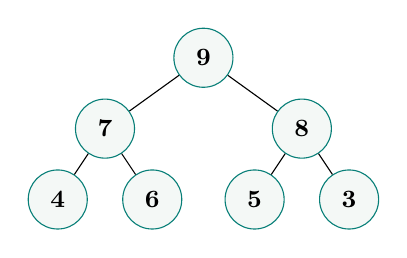
\begin{tikzpicture}[
 level distance=9mm,
 level 1/.style={sibling distance=25mm},
 level 2/.style={sibling distance=12mm},
 every node/.style={circle,draw=hbgreen,fill=hblight,minimum size=7.5mm,font=\small\bfseries}]
\node {9}
 child {node {7} child {node {4}} child {node {6}}}
 child {node {8} child {node {5}} child {node {3}}};
\end{tikzpicture}
\end{center}
\[
\begin{aligned}
parent(i)&=\left\lfloor(i-1)/2\right\rfloor\\
left(i)&=2i+1,\quad right(i)=2i+2
\end{aligned}
\]
\column{0.55\textwidth}
\footnotesize
\begin{block}{Thứ tự ưu tiên được đặc tả trước}
\begin{enumerate}
  \item điểm = lượt tăng $-$ lượt giảm, theo thứ tự giảm dần;
  \item số lượt tăng bình chọn giảm dần;
  \item \code{shuffleOrder} khi quản trị viên xáo thứ tự;
  \item \code{requestedAt} tăng dần để giữ nguyên tắc đến trước phục vụ trước.
\end{enumerate}
\end{block}
\begin{block}{Định vị $O(1)$ trung bình, tái cân bằng $O(\log n)$}
{\ttfamily\scriptsize
i = heap->index\_by\_id[id];\\
heap->items[i].score += delta;\\
delta > 0 ? heapify\_up(heap,i) : heapify\_down(heap,i);}
\end{block}
\smallskip
\end{columns}
\end{frame}

% 5 ---------------------------------------------------------------------------
\begin{frame}{Liên kết vòng loại bỏ trường hợp biên của chế độ lặp}
\small
\begin{center}
\begin{tikzpicture}[>=Stealth,node distance=11mm,
 box/.style={draw=hbnavy,fill=hblight,rounded corners=3pt,minimum width=25mm,minimum height=9mm,font=\bfseries}]
\node[box](a){Bài 1};
\node[box,right=of a](b){Bài 2};
\node[box,right=of b](c){Bài 3};
\draw[->,hbgreen,line width=1pt](a.north east)to[bend left=25](b.north west);
\draw[->,hbgreen,line width=1pt](b.north east)to[bend left=25](c.north west);
\draw[->,hbgreen,line width=1pt](c.east)to[bend left=42]node[above]{tiến}(a.west);
\draw[->,hbnavy](c.south west)to[bend left=25](b.south east);
\draw[->,hbnavy](b.south west)to[bend left=25](a.south east);
\draw[->,hbnavy](a.west)to[bend right=42]node[below]{lùi}(c.east);
\end{tikzpicture}
\end{center}
\vspace{-0.35cm}
\begin{columns}[T,totalwidth=\textwidth]
\column{0.47\textwidth}
\begin{block}{Thao tác con trỏ}
\begin{itemize}
  \item \code{current = current->next/prev}.
  \item \code{tail = head->prev}; \code{tail->next = head}.
\end{itemize}
\end{block}
\column{0.49\textwidth}
\begin{block}{Hệ quả}
\begin{itemize}
  \item Không cần nhánh riêng ở cuối danh sách.
  \item Bài lấy khỏi Heap được nối vào cuối lịch sử.
\end{itemize}
\end{block}
\end{columns}
\end{frame}

% 6 ---------------------------------------------------------------------------
\begin{frame}{Cửa sổ trượt chặn vi phạm trước khi hàng đợi bị thay đổi}
\begin{columns}[T,totalwidth=\textwidth]
\column{0.48\textwidth}
\begin{block}{Trạng thái lưu theo từng StudentID}
\begin{itemize}
  \item Các \code{songKey + timestamp} trong cửa sổ hiện hành;
  \item \code{activeRequestIds} đang sở hữu;
  \item \code{blockedUntil}, lý do và số lần vi phạm.
\end{itemize}
\end{block}
\begin{center}
\metricline{Tối đa 3 yêu cầu trong 10 phút \quad\textbullet\quad chặn 30 phút khi vi phạm}
\end{center}
\column{0.48\textwidth}
\begin{enumerate}
  \item Chuẩn hóa StudentID.
  \item Loại các mốc cũ ngoài cửa sổ 10 phút.
  \item Kiểm tra trạng thái chặn, bài trùng và hạn mức.
  \item Khi vi phạm: chụp tập ID, cập nhật trạng thái chặn và thu hồi khỏi Heap.
\end{enumerate}
\begin{alertblock}{Điểm quan trọng}
Hệ thống không chỉ từ chối yêu cầu mới mà còn thu hồi toàn bộ bài đang chờ của tài khoản vi phạm.
\end{alertblock}
\end{columns}
\end{frame}

% 7 ---------------------------------------------------------------------------
\begin{frame}{Backend C điều phối toàn bộ cấu trúc dữ liệu}
\begin{center}
\begin{tikzpicture}[>=Stealth,node distance=8mm and 10mm,font=\small,
 comp/.style={draw=hbnavy,fill=hblight,rounded corners=3pt,minimum width=32mm,minimum height=11mm,align=center},
 core/.style={draw=hbgreen,fill=hbgreen!7,rounded corners=3pt,minimum width=31mm,minimum height=10mm,align=center}]
\node[comp](ui){Giao diện React\\Quản trị + sinh viên};
\node[comp,right=of ui](state){PHP reverse proxy\\JSON command};
\node[comp,right=of state](sync){Backend C11\\nguồn sự thật};
\node[core,below=13mm of ui](heap){Max-Heap + Map chỉ số};
\node[core,right=of heap](cdll){Circular DLL};
\node[core,right=of cdll](spam){Hash Map SpamGuard};
\draw[->](ui)--(state);
\draw[<->](state)--(sync);
\draw[<->](sync)--(heap);
\draw[<->](sync)--(cdll);
\draw[<->](sync)--(spam);
\end{tikzpicture}
\end{center}
\vspace{0.35cm}
\begin{itemize}
  \item PHP không lưu state; mọi command được chuyển tới tiến trình C chạy tại cổng 8081.
  \item Các thẻ trình duyệt cùng đọc snapshot Max-Heap và CDLL do C xác nhận bất biến.
  \item Quản trị viên sở hữu trình phát và cấu hình; sinh viên chỉ tác động đến yêu cầu và bình chọn.
  \item Web App Manifest và service worker cho phép cài ứng dụng dưới dạng PWA.
\end{itemize}
\end{frame}

% 8 ---------------------------------------------------------------------------
\begin{frame}{Luồng yêu cầu, bình chọn và phát bài}
\begin{center}
\resizebox{0.96\textwidth}{!}{\begin{tikzpicture}[
  >=Stealth,
  font=\footnotesize\sffamily,
  flowstep/.style={
    draw=hbline,
    rounded corners=2pt,
    fill=white,
    minimum width=29mm,
    minimum height=10mm,
    align=center
  },
  decision/.style={
    diamond,
    draw=hbgreen,
    fill=hbgreen!6,
    aspect=2.05,
    minimum width=31mm,
    minimum height=12mm,
    align=center,
    inner sep=1pt
  },
  edge/.style={->,line width=0.45pt},
  answer/.style={font=\scriptsize\sffamily,fill=white,inner sep=1pt}
]
\node[flowstep] (request) at (0,0) {Sinh viên\\chọn bài};
\node[decision] (license) at (3.8,0) {Giấy phép\\hợp lệ?};
\node[decision] (guard) at (7.7,0) {SpamGuard\\cho phép?};
\node[flowstep] (heap) at (11.5,0) {Thêm / bình chọn\\heapify};

\node[flowstep] (reject) at (3.8,-2.05) {Từ chối\\ghi nhật ký};
\node[flowstep] (block) at (7.7,-2.05) {Chặn 30 phút\\thu hồi yêu cầu};
\node[flowstep] (extract) at (11.5,-2.05) {Quản trị Next\\extractMax};

\node[flowstep] (audit) at (3.8,-4.1) {Nhật ký +\\đồng bộ giao diện};
\node[flowstep] (history) at (7.7,-4.1) {Phát + addLast\\vào CDLL};

\draw[edge] (request.east) -- (license.west);
\draw[edge] (license.east) -- node[answer,above]{có} (guard.west);
\draw[edge] (guard.east) -- node[answer,above]{có} (heap.west);
\draw[edge] (license.south) -- node[answer,right]{không} (reject.north);
\draw[edge] (guard.south) -- node[answer,right]{không} (block.north);
\draw[edge] (heap.south) -- (extract.north);
\draw[edge] (extract.south) -- ++(0,-5mm) -| (history.east);
\draw[edge] (history.west) -- (audit.east);
\draw[edge] (reject.south) -- (audit.north);
\draw[edge] (block.south) -- ++(0,-5mm) -| (audit.east);
\end{tikzpicture}
}
\end{center}
\vspace{0.06cm}
\begin{center}
\metricline{Kiểm tra quyền trước \quad\textbullet\quad chặn vi phạm trước khi sửa Heap
\quad\textbullet\quad phát bài rồi nối vào CDLL}
\end{center}
\end{frame}

% 9 ---------------------------------------------------------------------------
\begin{frame}{Quyền phát được kiểm tra ở cả giao diện và tầng xử lý}
\small
\begin{columns}[T,totalwidth=\textwidth]
\column{0.50\textwidth}
\begin{block}{Một bài được mở khi}
\[
\begin{aligned}
approved \land publicPlaybackAllowed\\[-2pt]
\land\ licenseUrl \ne \varnothing
\end{aligned}
\]
\begin{itemize}
  \item Giao diện vô hiệu hóa nút yêu cầu.
  \item Backend C chỉ chấp nhận mã bài thuộc danh mục cố định.
  \item Quản trị viên xem nguồn, giấy phép và thông tin ghi công.
\end{itemize}
\end{block}
\column{0.46\textwidth}
\begin{itemize}
  \item Gói phát hành dùng 18 file piano MP3 do chủ dự án cung cấp.
  \item Thông tin ghi công được đọc từ ID3 và lưu trong danh mục.
  \item Openverse/Jamendo chỉ là nguồn tìm kiếm tương lai; từng mục vẫn phải được xác minh.
  \item Không tải, lưu đệm hoặc chuyển đổi nội dung từ Spotify, Apple Music hay YouTube.
\end{itemize}
\end{columns}
\vspace{0.1cm}
\begin{center}
\metricline{Khóa mặc định \quad\textbullet\quad ghi công \quad\textbullet\quad nhật ký
\quad\textbullet\quad 18 bản piano MP3 cục bộ}
\end{center}
\end{frame}

% 10 --------------------------------------------------------------------------
\begin{frame}{Giao diện làm rõ mối liên hệ giữa gốc Heap và bài kế tiếp}
\begin{center}
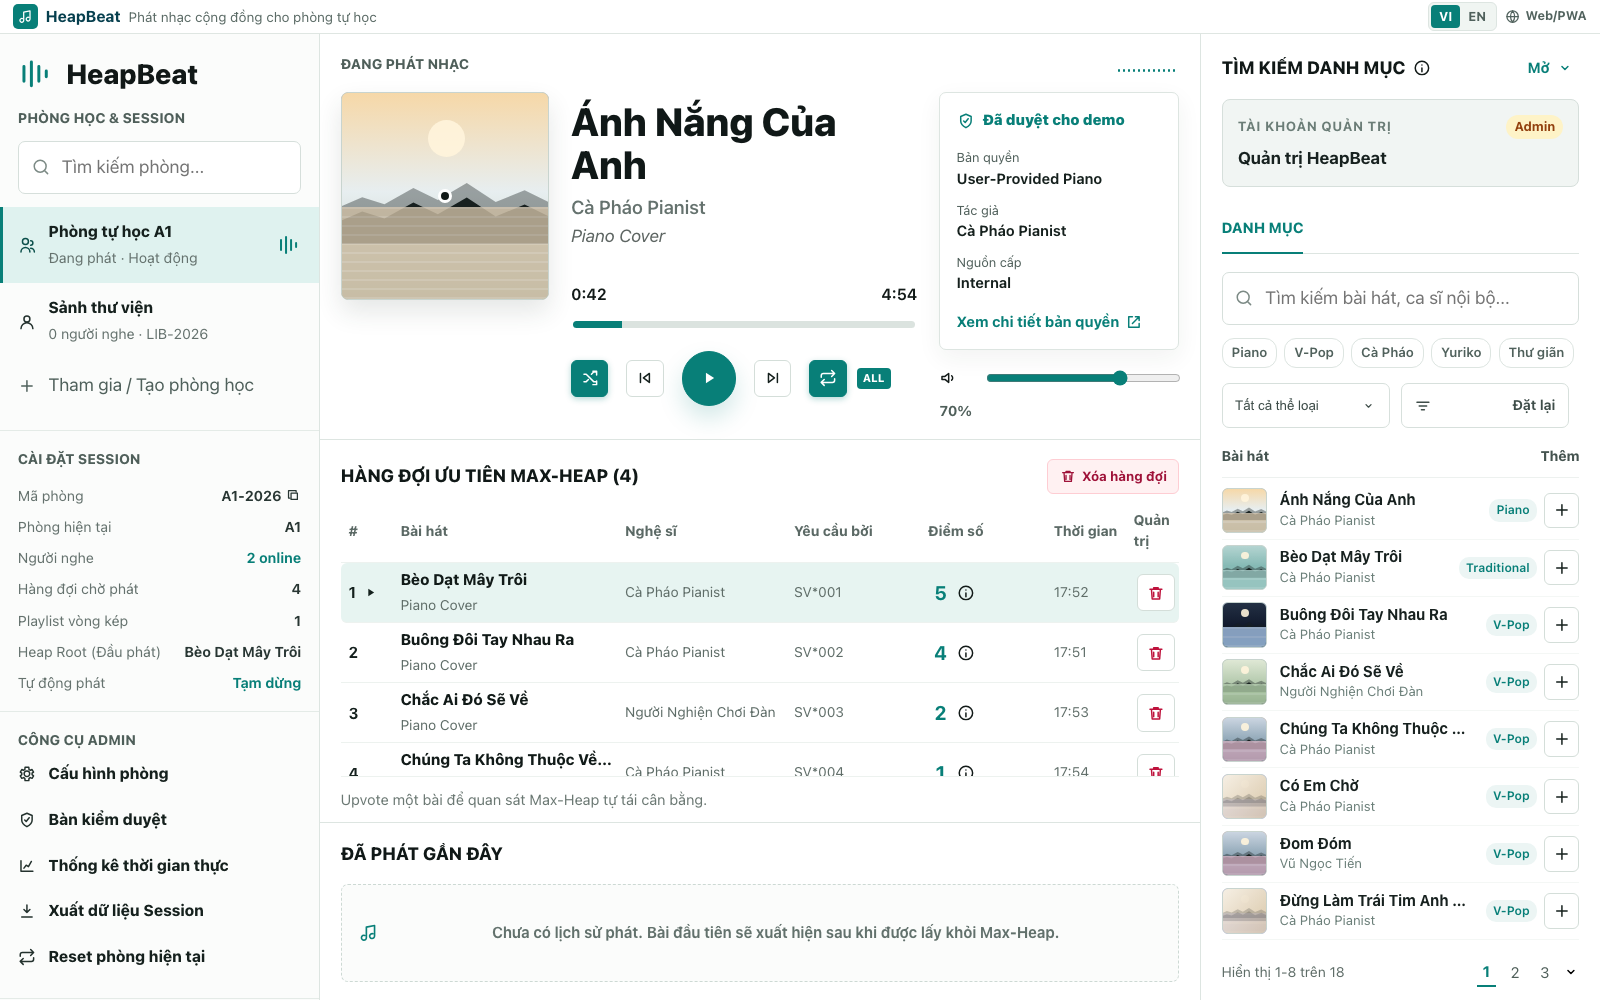
\includegraphics[height=5.25cm,keepaspectratio]{../report/screenshot-desktop.png}
\end{center}
\vspace{-0.08cm}
\begin{center}
\metricline{Phòng học \quad\textbullet\quad bài đang phát \quad\textbullet\quad gốc Heap
\quad\textbullet\quad danh mục \quad\textbullet\quad kiểm duyệt}
\end{center}
\end{frame}

% 11 --------------------------------------------------------------------------
\begin{frame}{Kết quả kiểm thử nhất quán với các bất biến đã đặc tả}
\small
\begin{columns}[T,totalwidth=\textwidth]
\column{0.46\textwidth}
\begin{block}{Kiểm thử đơn vị: 22/22 đạt}
\begin{itemize}
  \item Circular DLL: 4/4
  \item QueueMaxHeap: 7/7
  \item SpamGuard: 5/5
  \item Trạng thái phát: 4/4
  \item Danh mục MP3 và đường dẫn: 2/2
\end{itemize}
\end{block}
{\sffamily\small\bfseries\color{hbgreen}Định dạng đạt \textbullet\ bản dựng web đạt
\textbullet\ C11 với Werror đạt}
\column{0.50\textwidth}
\begin{center}
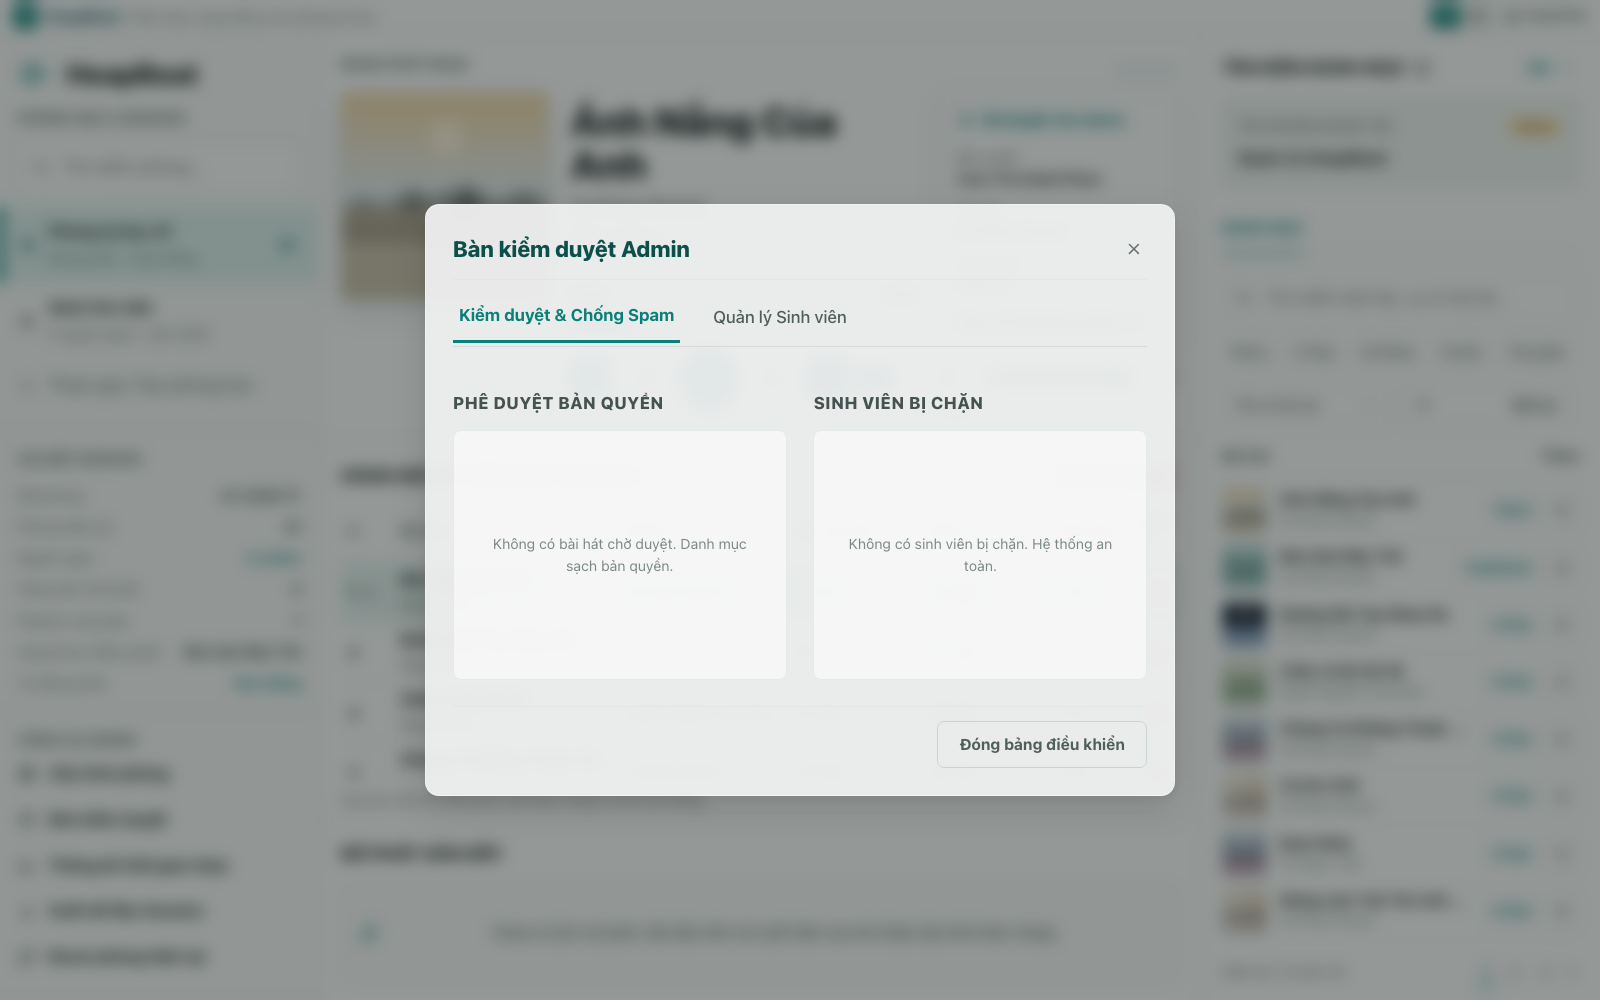
\includegraphics[height=2.78cm,keepaspectratio]{../report/screenshot-moderation.png}
\end{center}
\vspace{-0.06cm}
\begin{itemize}
  \item Bình chọn đổi điểm 4$\to$5 và thay đổi gốc Heap.
  \item Yêu cầu trùng chặn SV9999 và thu hồi đúng bài.
  \item Next/Previous đi đúng vòng lịch sử; trình phát không phát sinh lỗi.
\end{itemize}
\end{columns}
\end{frame}

% 12 --------------------------------------------------------------------------
\begin{frame}{Max-Heap phù hợp với luồng bình chọn thay đổi liên tục}
\small
\begin{tabularx}{\textwidth}{@{}lcccX@{}}
\toprule
\textbf{Phương án} & \textbf{Xem đầu} & \textbf{Thêm} & \textbf{Đổi bình chọn} & \textbf{Nhận xét}\\
\midrule
Mảng chưa sắp xếp & $O(n)$ & $O(1)$ & $O(1)$ & Phát bài phải quét.\\
Mảng luôn sắp xếp & $O(1)$ & $O(n)$ & $O(n)$ & Bình chọn làm dịch chuyển phần tử.\\
Cây cân bằng & $O(\log n)$ & $O(\log n)$ & $O(\log n)$ & Phức tạp hơn phạm vi nguyên mẫu.\\
\alert{Max-Heap + Map} & $O(1)$ & $O(\log n)$ & $O(\log n)$ &
Cân bằng hiệu năng, bộ nhớ, khả năng minh họa.\\
\bottomrule
\end{tabularx}
\vspace{0.45cm}
\begin{columns}[T,totalwidth=\textwidth]
\column{0.48\textwidth}
\begin{block}{Điểm mạnh}
CTDL hiện rõ trên giao diện; kiểm thử độc lập; phân giải đồng hạng ổn định; thu hồi theo ID.
\end{block}
\column{0.48\textwidth}
\begin{block}{Giới hạn đo lường}
Chưa đo với hàng nghìn yêu cầu; lưu trữ tệp chưa phù hợp với tải đồng thời lớn.
\end{block}
\end{columns}
\end{frame}

% 13 --------------------------------------------------------------------------
\begin{frame}[plain]
\begin{tikzpicture}[remember picture,overlay]
  \fill[white](current page.south west)rectangle(current page.north east);
  \fill[hbnavy](current page.south west)rectangle($(current page.north west)+(0.28cm,0)$);
  \fill[hblight](current page.south west)rectangle($(current page.south east)+(0,0.18\paperheight)$);
  \fill[hbgreen](current page.south west)rectangle($(current page.south east)+(0,0.025\paperheight)$);
\end{tikzpicture}
\centering\color{hbnavy}
\vspace{0.38cm}
{\scriptsize\bfseries\color{hbgreen}KẾT LUẬN VÀ KIỂM CHỨNG\par}
\vspace{0.1cm}
{\fontsize{25}{29}\selectfont\bfseries Ba cấu trúc dữ liệu tạo thành\\một Collaborative DJ Queue nhất quán\par}
\vspace{0.22cm}
{\large Max-Heap \textbullet\ danh sách liên kết đôi vòng \textbullet\ Hash Map\par}
\vspace{0.62cm}
\begin{columns}[c,totalwidth=0.88\textwidth]
\column{0.54\textwidth}
\raggedright
{\scriptsize\bfseries\color{hbgreen}BẢN DEMO\par}
\vspace{0.12cm}
{\small\href{https://phamhungtien.synology.me/heapbeat/}{phamhungtien.synology.me/heapbeat/}\par}
\vspace{0.08cm}
{\small Tài khoản demo: \code{admin / admin@123}\par}
\column{0.30\textwidth}
\centering
\href{https://phamhungtien.synology.me/heapbeat/}{%
  \qrcode[height=2.35cm]{https://phamhungtien.synology.me/heapbeat/}}
\par\vspace{0.08cm}
{\scriptsize\bfseries\color{hbgreen}QUÉT ĐỂ MỞ BẢN DEMO\par}
\end{columns}
\vfill
\end{frame}

\end{document}
